\subtitle{Modelos Gaussianos}
 \begin{frame}{}
     \maketitle
 \end{frame}

%\section{Resolución de ecuación de transporte}
\begin{frame}{Resolución de la ecuación de transporte}

    Modelar la química atmosférica consiste en resolver la \alert{ecuación de transporte}:\footnote{$c$: concentración de especie quimica, $v$: velocidad del viento, $K$: coeficiente de turbulencia, $E$: tasa de emisión, $\lambda$: constante de reacción/degradación.}
    
    $$
    \dfrac{\partial c}{\partial t}  
    =
    \underbrace{E }_{\text{Emisión}}
    -
    \underbrace{\lambda \,c}_{\text{Química}}
    -
    \underbrace{u \dfrac{\partial c}{\partial x}  }_{\text{Advección}}
    +
    \underbrace{K \dfrac{\partial^2 c}{\partial x^2} }_{\begin{smallmatrix}\text{Mezclado}\\ \text{turbulento} \end{smallmatrix}}
    $$
    
    Expresa la \textit{conservación de masa} para una especie $c$ transportado por la atmósfera.\\[.5em]

\pause

Hay dos caminos para resolverla:
\begin{columns}
\column{0.5\textwidth}
    \begin{exampleblock}{Analítico}
        \begin{itemize}
            \item Solución exacta. 
            \item Utiliza supuestos y simplificaciones.
            \item Muy rápidos de computar.
        \end{itemize}
    \end{exampleblock}
    
\column{0.5\textwidth}
    \begin{alertblock}{Numérico}
        \begin{itemize}
            \item Solución aproximada.
            \item Sin supuestos ni simplificaciones.
            \item Demandan mucho poder de cálculo.
        \end{itemize}
    \end{alertblock}
\end{columns}
\end{frame}

\section{Solución Analítica a Ecuación de Transporte}
\begin{frame}{Solución Analítica}{Modelos Gaussianos}

Dan la solución a: %\footnote{Desprecia advección en $y$ y $z$}

$$
\dfrac{\partial c}{\partial t} = - u \dfrac{\partial c}{\partial x}+K_x\dfrac{\partial^2 c}{\partial x^2}  
$$

\pause
Cuya solución analítica tiene la forma:\footnote{$\mu= u t$, $\sigma_x=\sqrt{2K_xt}$}

$$c_{(x,t)}=\frac{M}{\sqrt{2\pi } \sigma_{x} } \exp \bigg[ - \frac{1}{2} \frac{ (x-\mu)^2}{\sigma_x^2}  \bigg]$$

\pause
\centering
\begin{center}
\begin{tikzpicture}[baseline=(current bounding box.center),font=\small]
    \begin{axis}[%no markers,
      domain=-3:2, samples=60,
      axis lines*=left, xlabel=$x$, ylabel=$c_{(x)}$,
      height=3cm, width=6cm,
      xtick=\empty, ytick=\empty,
      enlargelimits=false, clip=false, axis on top,
      grid = major
      ]
      \addplot [very thick,color=blue!70,fill=blue!40,text=black!80] {gauss(-1,.5)};%,cyan!50!black,fill=cyan!50!black!20
      \draw [|-|,thick,red!80](-1,0) -- node [midway,anchor=north] {$\sigma$} (-.5,0);
      \draw [dotted,red!80](-1,0) --  (-1,1.) node {$\mu$};
    \end{axis}
\end{tikzpicture}
\end{center}
%\begin{tikzpicture}[baseline=(current bounding box.center)]
%    \begin{axis}[%no markers,
%      domain=-3:5, samples=100,
%      axis lines*=left, xlabel=$x$, ylabel=$c_{(x)}$,
%      height=3cm, width=6cm,
%      xtick=\empty, ytick=\empty,
%      enlargelimits=false,
%      clip=false, axis on top,
%           ylabel near ticks, ylabel shift={4pt},xlabel near ticks, xlabel shift={4pt},
%      ]
%      \addplot [very thick,blue!50,fill=blue!50] {gauss(-1,.5)};
%      \addplot [dashed, very thick,blue!50,fill=blue!50,opacity=0.5] {gauss(2,1)};
%          
%      \draw[|-|,very thick](-1,0) -- node [midway,anchor=north] {\small$\sigma$} (-.5,0);
%      \draw[dotted](-1,0)--(-1,1.) node {\small$\mu$};
%      \draw[-latex,red!75](-1,0.5)--(2,.5) node [midway,anchor=south] {\small$\vec{u}\Delta t$};
%      \draw[dotted](2,0)--(2,1.0) node {\small$\mu + u \Delta t$};
%    
%    \end{axis}
%\end{tikzpicture}

\end{frame}


\begin{frame}{Intuición solución analítica}
    
    Graficar solución analítica:
    
    \begin{center}
    \Large
        \href{https://www.desmos.com/calculator}{https://www.desmos.com/calculator}
    \end{center}
    
    Discusión:
    \begin{itemize}
        \item  Interpretar parámetros ($\mu$ y $\sigma$).
        \item Representa difusión?
        \item Representa advección?
        \item Garantiza conservación de masa?
        \item Incluir término de decaimiento.
    \end{itemize}
    
\end{frame}

\section{Puff Gaussiano}

\begin{frame}{Puff Gaussiano}{Solución \alert{transitoria} }

Resuelve:   
$$ \dfrac{\partial c}{\partial t} = - u \dfrac{\partial c}{\partial x} + K_x\dfrac{\partial^2 c}{\partial x^2} +K_y\dfrac{\partial^2 c}{\partial y^2} +K_z\dfrac{\partial^2 c}{\partial z^2} $$

\pause

Cuya solución es\footnote{$\mu= u t$, $\sigma_{*}=\sqrt{2K_{*}t}$}:
     $$\begin{array}{ll}
     C_{(x,y,z,t)} = & \dfrac{M}{\sqrt{2\pi}^3\sigma_x\sigma_y\sigma_z} \exp \bigg[ - \dfrac{(x-ut)^2}{2\sigma_x^2} \bigg] \exp \bigg[ -\dfrac{y^2}{2\sigma_y^2} \bigg] \exp \bigg[ - \dfrac{z^2}{2\sigma_z^2} \bigg] 
     \end{array}
     $$

\pause
%Here begins the 3D plot
\begin{center}
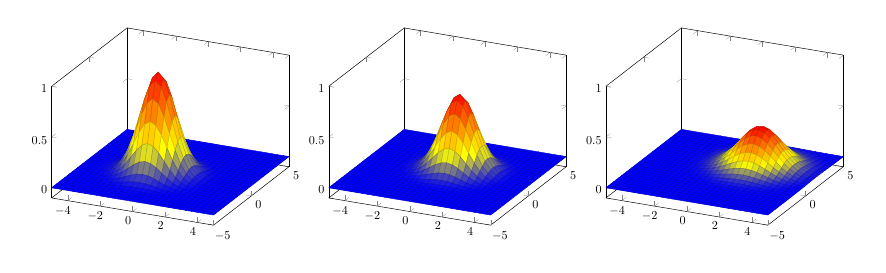
\begin{tikzpicture}[scale=0.44]
    \begin{axis}[xshift=-4cm,zmax=1]
        \addplot3[surf,samples=30]{1.00*exp(-(y+0.5)^2/2)*exp(-(x+0.5)^2/2)};
    \end{axis}
    \begin{axis}[xshift=4cm,zmax=1.0]
        \addplot3[surf,samples=30]{0.75*exp(-(y-0.5)^2/2)*exp(-(x-0.5)^2/2)};
    \end{axis}
    \begin{axis}[xshift=12cm,zmax=1.0]
        \addplot3[surf,samples=30]{0.40*exp(-(y-1.5)^2/3)*exp(-(x-1.5)^2/3)};
    \end{axis}
\end{tikzpicture}
\end{center}
%Here ends the 3D plot
\end{frame}

%\begin{frame}{Puff Gaussiano}{Supuestos}
%    
%\end{frame}



\section{Pluma Gaussiana}

\begin{frame}{Pluma Gaussiana}{Solución \alert{estacionaria}}

Si planteamos la condición de equilibrio:\footnote{Despreciamos la mezcla turbulenta en $x$ ya que es muy chico comparado con la advección.}
$$
\dfrac{\partial c}{\partial t} =0= - u \dfrac{\partial c}{\partial x}  +K_y\dfrac{\partial^2 c}{\partial y^2} +K_z\dfrac{\partial^2 c}{\partial z^2} $$

Despejando:
$$  \dfrac{\partial c}{\partial x} =  \dfrac{K_{y}}{u} \dfrac{\partial^2 c}{\partial y^2}  +\dfrac{K_{z}}{u} \frac{\partial^2 c}{\partial z^2} $$
\end{frame}

\begin{frame}{Pluma Gaussiana}{Solución \alert{estacionaria}}
 
Resuelve:
$$  \dfrac{\partial c}{\partial x} =  \dfrac{K_{y}}{u} \dfrac{\partial^2 c}{\partial y^2}  +\dfrac{K_{z}}{u} \frac{\partial^2 c}{\partial z^2} $$
 
\pause

Cuya solución es:\footnote{Dado que $t = x/u = cte.$, entonces:  $\sigma_i=\sqrt{2K_i t}=\sqrt{2 K_i x/u}$.}

$$
c_{(x,y,z)} = \dfrac{Q}{u\sqrt{2\pi}^2\sigma_y\sigma_z} \exp \bigg[ -\dfrac{y^2}{2\sigma_y^2} \bigg] \exp \bigg[ - \dfrac{z^2}{2\sigma_z^2} \bigg] 
$$
     
\pause
%Here begins the 3D plot
\begin{center}
\begin{tikzpicture}[scale=0.45]
    \begin{axis}[xshift= -5cm,domain=0.01:15,
        y domain=-10:10]%,xmin=0.01,ymin=-10,ymax=10]%,zmax=1]
        \addplot3[contour filled={number=13}, samples=60]{1.00/sqrt(x)*exp(-(y)^2/x)};
    \end{axis}
    \begin{axis}[xshift= 5cm,domain=0.01:15,
        y domain=-10:10,view={0}{90}]%,xmin=0.01,ymin=-10,ymax=10]%,zmax=1]
        \addplot3[contour filled={number=13}, samples=90]{1.00/sqrt(x)*exp(-(y)^2/x)};
    \end{axis}
\end{tikzpicture}
\end{center}
%Here ends the 3D plot
\end{frame}

%\begin{frame}{Pluma Gaussiana}{Supuestos}
%    
%\end{frame}

\begin{frame}{Comparación Pluma Gaussiana con experimento de Richardson}

\begin{center}
\begin{tikzpicture}[scale=0.45]
 \node[opacity=1.,inner sep=1pt] (image) at (current page.center){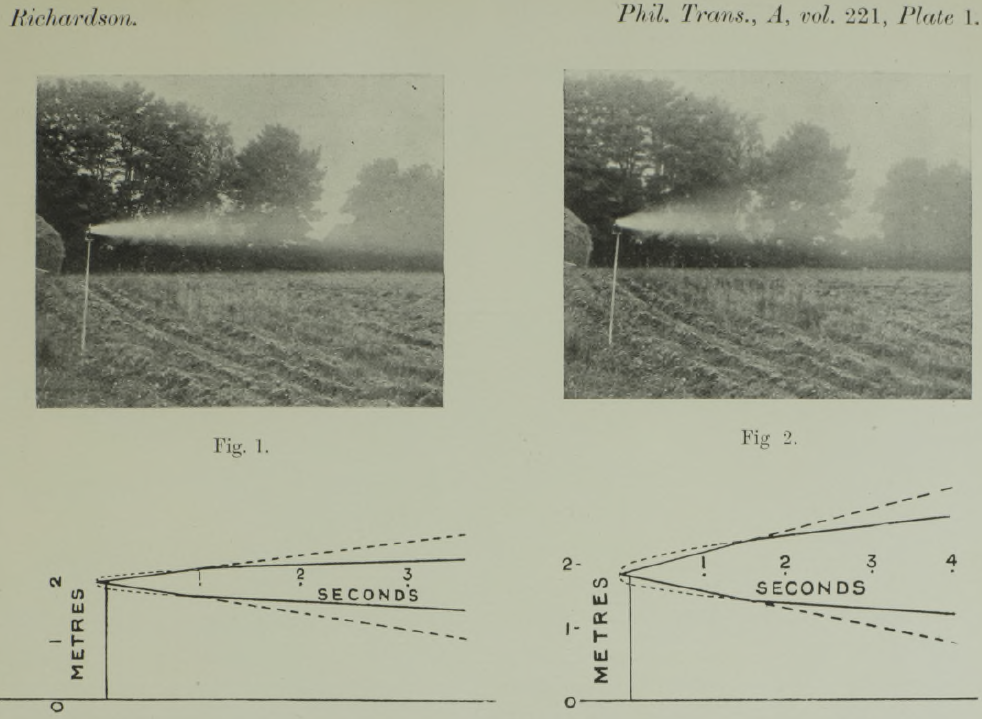
\includegraphics[width=0.65\textwidth]{img/richardsonPlumas-1921.png}};
\end{tikzpicture}
\end{center}

\end{frame}
%
%
%\section{Modificacciones a modelo Gaussiano}
%
%%\begin{frame}{Descomposición de operadores}
%%    
%%    
%%    $$c_{(x,y,z)} = \frac{Q}{u}\, \Phi_x \Phi_y \Phi_z  $$
%%    
%%    donde:
%%    $$\Phi_x = 1 $$
%%    $$\Phi_y = \dfrac{1}{\sqrt{2\pi} \sigma_y}\exp{\bigg( \dfrac{y^2}{2\sigma_y^2}\bigg)}$$
%%    $$\Phi_z = \dfrac{1}{\sqrt{2\pi} \sigma_z}\exp{\bigg( \dfrac{z^2}{2\sigma_z^2}\bigg)}$$
%%    
%%\end{frame}
%
%
%\begin{frame}[t]{Altura de la fuente}
%    \centering
%\begin{tikzpicture}[scale=1.3]
%     \clip(-4,-1) rectangle (4,2);
%%axis:
%\ejesXZ{-5}{0}{0.45}
%%piso
%\piso{-4}{4.5}{0}
%\chimenea{-3.1}{0}{0.2}{1.2}
%%\draw[fill=black!60](#1,#2) rectangle ++(#3,#4);
%%\node(chim1)[fill=black!60,minimum height=1.25cm] at (-3.1,0.6){};
%%\fill[red!20,opacity=0.5] (chim1.north) -- (4,2) -- (4,-1) -- (chim1.north);
%\fill[red!20,opacity=0.5] (-3.1,1.2) -- (4,2) -- (4,-1) -- (-3.1,1.2);
% 
%\draw[| latex-latex] (-3.2, 1.2)--(-3.2,0) node[midway, anchor=east]{$H$};
% 
%\end{tikzpicture}
% 
%     $$\begin{array}{ll}
%     C_{(x)} = & \dfrac{Q}{u\sqrt{2\pi}^2\sigma_y\sigma_z} \exp \bigg[ -\dfrac{y^2}{2\sigma_y^2} \bigg] \exp \bigg[ - \dfrac{(z\alert{-H})^2}{2\sigma_z^2} \bigg] 
%     \end{array}
%     $$
% 
%\end{frame}
% \begin{frame}{Altura efectiva}{Plume Rise}
% 
%\begin{center}
%\begin{tikzpicture}[scale=1.3]
%     \clip(-4,-0.5) rectangle (4,2);
% \ejesXZ{-5}{0}{0.45}
% \piso{-4}{4.5}{0}
% \chimenea{-3.1}{0}{0.2}{1.2}
%  %pluma real
% \fill[red!20,opacity=0.5] (-3.1,1.75) -- (4,2) -- (4,0.5) -- (-3.1,1.75);
%  \draw[| latex-latex] (-3.2, 1.2)--(-3.2,0) node[midway, anchor=east]{$H$};
%  \draw[| latex-latex] (-3.2, 1.2)--(-3.2,1.75) node[midway, anchor=east]{$\Delta h$};
%  \end{tikzpicture}
% \end{center}  
%
%Elevación por empuje térmico y e impulso en la fuente.
%  
%    $$
%    C_{(x)} = \dfrac{Q}{u\sqrt{2\pi}^2\sigma_y\sigma_z} \exp \bigg[ -\dfrac{y^2}{2\sigma_y^2} \bigg] \exp \bigg[ - \dfrac{(z-H - \alert{\Delta h})^2}{2\sigma_z^2} \bigg] 
%    $$
% 
% \end{frame}
% 
% 
% 
% 
%\begin{frame}[t]{Edificios y obstaculos}{Downwash}
%
%\begin{center}
%\begin{tikzpicture}[scale=1.3]
%     \clip(-4,-0.5) rectangle (4,2);
%%axis:
%\ejesXZ{-5}{0}{0.45}
%%piso
%\piso{-4}{4.5}{0}
%%pluma real
%\chimenea{-3.1}{0}{0.2}{1.2}
%\fill[red!20,opacity=0.5] (-3,1.2) --(0,1.4)to[out=0,in=182] (4,1.2) -- (4,0) to[out=180, in=-5] (0,1) -- (-3,1.2);
% 
%\draw[| latex-latex] (-3.2, 1.2)--(-3.2,0) node[midway, anchor=east]{$H$};
% 
%\draw[building](0,0) rectangle (0.5,0.8);
% 
%%remolinos
%\draw [>=stealth,->,blue!80] (0.7,0.1) arc (280:0:.1cm) -- +(283:0.05cm);
%\draw [>=stealth,->,blue!80] (0.7,0.3) arc (280:0:.1cm) -- +(283:0.05cm);
%\draw [>=stealth,->,blue!80] (0.7,0.6) arc (280:0:.1cm) -- +(283:0.05cm);
%\draw [>=stealth,->,blue!80] (1.0,0.2) arc (280:0:.1cm) -- +(283:0.05cm);
%\draw [>=stealth,->,blue!80] (1.0,0.5) arc (280:0:.1cm) -- +(283:0.05cm);
%\draw [>=stealth,->,blue!80] (1.3,0.4) arc (280:0:.1cm) -- +(283:0.05cm);
%\draw [>=stealth,->,blue!80] (1.3,0.1) arc (280:0:.1cm) -- +(283:0.05cm);
%\draw [>=stealth,->,blue!80] (1.6,0.2) arc (280:0:.1cm) -- +(283:0.05cm);
%\draw [>=stealth,->,blue!80] (1.9,0.1) arc (280:0:.1cm) -- +(283:0.05cm);
% 
%\end{tikzpicture}
%\end{center} 
% 
% Deflección por sombra turbulenta generada por edificios y obstaculos:
%    $$
%    C_{(x)} = \dfrac{Q}{u\sqrt{2\pi}^2\sigma_y\sigma_z} \exp \bigg[ -\dfrac{y^2}{2\sigma_y^2} \bigg] \exp \bigg[ - \dfrac{(z-H - \alert{\Delta h})^2}{2\sigma_z^2} \bigg] 
%    $$
%\end{frame}
%
%
%\begin{frame}[t]{Terreno (plano)}{Reflexión}
%    \centering
%\begin{tikzpicture}%[scale=1.3]
%    \clip(-4,-2.0) rectangle (4,2);
%%axis:
%\ejesXZ{-5}{0}{0.45}
%%piso
%\piso{-4}{4.5}{0}
%\node(chim1)[fill=black!60,minimum height=1.25cm] at (-3,0.6){};
%\node(chim2)[fill=black!60,minimum height=1.25cm,opacity=0.5] at (-3,-0.6){};
%
%\fill[red!20,opacity=0.5] (chim1.north) -- (4,2) -- (4,-1) -- (chim1.north);
%\fill[blue!20, opacity=0.3, pattern=north east lines] (chim2.south) -- (4,-2) -- (4,1) -- (chim2.south);
%
%\fill[pattern=north east lines,pattern color=red] (0.8,0) -- (4,0) -- (4,1) --(0.8,0);
%
%\draw[| latex-latex] (-3.2, 1.2)--(-3.2,0) node[midway, anchor=east]{$H$};
%\draw[| latex-latex,opacity=0.5] (-3.2,-1.2)--(-3.2,0) node[midway, anchor=east]{$-H$};
%
%\end{tikzpicture}
% 
%     $$\begin{array}{ll}
%     C_{(x)} = & \dfrac{Q}{u\sqrt{2\pi}^2\sigma_y\sigma_z} \exp \bigg[ -\dfrac{y^2}{2\sigma_y^2} \bigg] \bigg(\exp \bigg[ - \dfrac{(z-H)^2}{2\sigma_z^2} \bigg] \alert{+ \exp \bigg[ - \dfrac{(z+H)^2}{2\sigma_z^2} \bigg]}\bigg)
%     \end{array}
%     $$
% 
%\end{frame}
%
%
%
%
%\begin{frame}[t]{Terreno complejo}{}
% 
%\centering
%\begin{tikzpicture}[scale=1.3]
%\ejesXZ{-5}{0}{0.45}
%\piso{-4}{4.5}{0}
%\chimenea{-3.1}{0}{0.2}{1.2}
%%pluma real
%\fill[red!20,opacity=0.5] (-3,1.2) -- (4,2.2) -- (4,0.4) -- (-3,1.2);
%%mountain
%\draw[ latex-latex] (-3.2, 1.2)--(-3.2,0) node[midway, anchor=east]{$H$};
%
%     \node[brown] at (0.5,0.8) {\textbullet};
%     \fill[fill=blue] (0.5,1.1) circle[radius=2pt] node[anchor=south west]{$r_1$};
%     \fill[fill=red ] (0.5,0.3) circle[radius=2pt] node[anchor=south west]{$r_2$};
%     
%     \draw[latex-latex] (1.0,0.0)--(1.0,0.8)node[midway,anchor=west]{$z_{t}$}; 
%     \draw[latex-latex] (0.5,0.8)--(0.5,1.1)node[midway,anchor=west]{$z_{p}$}; 
%     \draw[latex-latex] (0.5,0.0)--(0.5,0.3)node[midway,anchor=west]{$z_{p}$}; 
%     \draw[latex-latex] (1.5,0.0)--(1.5,1.1)node[midway,anchor=west]{$z_{r}$};
%     
%     \draw[orange!70, dashed] (-3,0.85)--(4,0.85) node[anchor=west]{$H_c$};
%   \draw[|-|, green] (4.5,0.85)--(4.5,2.2) node[midway, anchor=west]{$M_a$};
%   \draw[|-|, green] (4.5,0.85)--(4.5,0.5) node[midway, anchor=west]{$M_b$};
%   \draw[clip]
%    decorate [decoration={random steps,segment length=3pt,amplitude=1pt}]%
%    {(-1,0) --(0,0.3)-- (0.5,0.8) -- (1,1.5)--(2,2) --(3.0,2.5)-- (3.5,2.3) -- (4,0)}-- (0,0) -- (-1,0);
%    \fill[rock](-1,0) rectangle (4,4);
%        
%\end{tikzpicture}
%
%Se calculan dos plumas, una ignorando el terreno y otra siguiendo el terreno:
%
%$$ C_{tot} = f {\color{blue} C_{ref} } + (1-f) {\color{red}C_{terr.} } $$
%
%El resultado es una ponderación de estas dos determinadas por el factor $f$.
%
%
%\footnote{donde $f=0.5 + 0.5 \varphi_p $ y $\varphi_p= M_b / M_a\,M_b$. $M_a$ Masa sobre $H_c$ y $M_b$ masa por debajo de $H_c$. $h_c$: hill slope scale. $H_c$: critical dividing streamline}
%
%\end{frame}
%
%
%
%
%\begin{frame}{Coeficientes turbulentos}{Estabilidad}
%
%La estabilidad da idea de la libertad que tienen las maasas de aire para moverse verticalmente.
%
%\begin{center}
%\begin{tikzpicture}[scale=0.6]
%
%\begin{scope}[yshift=3cm]
%\ejesXZ{-5}{0}{0.45}
%\piso{-4}{4.5}{0}
%\chimenea{-3.1}{0}{0.2}{1.2}
% %pluma real
%\fill[red!20,opacity=0.5] (-3,1.2) -- (4,2.5) -- (4,0) -- (-3,1.2);
%\node[] at (6,1.2){Inestable};
%\end{scope}
%
%\begin{scope}[yshift=0cm]
%\ejesXZ{-5}{0}{0.45}
%\piso{-4}{4.5}{0}
%\chimenea{-3.1}{0}{0.2}{1.2}
% %pluma real
%\fill[red!20,opacity=0.5] (-3,1.2) -- (4,2) -- (4,0.5) -- (-3,1.2);
%\node[] at (6,1.2){Neutro};
%\end{scope}
%
%\begin{scope}[yshift=-3cm]
%\ejesXZ{-5}{0}{0.45}
%\piso{-4}{4.5}{0}
%\chimenea{-3.1}{0}{0.2}{1.2}
% %pluma real
%\fill[red!20,opacity=0.5] (-3,1.2) -- (4,1.5) -- (4,1.0) -- (-3,1.2);
%\node[] at (6,1.2){Estable};
%\end{scope}
%
%\end{tikzpicture}
%\end{center}
%
%\end{frame}
% 
%\begin{frame}{Coeficientes turbulentos}{Parametrizaciones basadas en clases de estabilidad}
%La clasificación mas usada para determinar la estabilidad atmosférica es la desarrollada por Pasquill (1961) y Gifford (1961). Ellos definieron 6 clases (A-F)\footnote{donde A: muy inestable, B: moderadamente estable, C: levemente estable, D neutral, E levemente estable, F: estable.}
% 
%\begin{table}[]
%    \centering
%\begin{tabular}{| c | c c c | c c |}
%\hline
%& \multicolumn{3}{c|}{Día} & \multicolumn{2}{c|}{Noche} \\
%& \multicolumn{3}{c|}{Radiación solar} & \multicolumn{2}{c|}{Nubosidad} \\
%$u (m/s)$ & Fuerte & Media & Débil & Nublado ($> 4/8$) & Despejado ($<3/8$) \\ \hline
%<2  & A   & A-B  & B & E & F \\ 
%2-3 & A-B & B    & C & E & F \\ 
%3-5 & B   & B-C  & C & D & E \\ 
%5-6 & C   & C-D  & D & D & D \\ 
%>6  & C   & D    & D & D & D \\ \hline
%\end{tabular}
%    \caption{Clases de Estabilidad}
%    \label{tab:my_label}
%\end{table}
%\end{frame}
%
% 
% 
% \begin{frame}{Coeficientes turbulentos}{Parametrizaciones basadas en clases de estabilidad}
%  
% Briggs (1973), propuso formulas empiricas para el calculo de los $\sigma$:
%  
% $$
% \sigma_y =\dfrac{a x}{(1+bx)^c}
% \qquad
% \sigma_z =\dfrac{d x}{(1+ex)^f}
% $$
%  
% Los coeficientes (a,b,c,d,e,f) están tabulados y dependen de la clase de estabilidad:
%  
%{\tiny
% \begin{columns}[t]
%
% 
% \column{0.5\textwidth}
% \begin{table}
%     \centering
% \begin{tabular}{| c | c c  c | c c c |}
% \hline
% C.E&    a &    b   &    c &     d &   e    & f  \\\hline
%  A & 0.22 & 0.0001 &  0.5 & 0.2   & 0      & —  \\     
%  B & 0.16 & 0.0001 &  0.5 & 0.12  & 0      & —  \\
%  C & 0.11 & 0.0001 &  0.5 & 0.08  & 0.0002 & 0.5\\
%  D & 0.08 & 0.0001 &  0.5 & 0.06  & 0.0015 & 0.5\\
%  E & 0.06 & 0.0001 &  0.5 & 0.03  & 0.0003 & 1  \\
%  F & 0.04 & 0.0001 &  0.5 & 0.016 & 0.0003 & 1  \\ \hline
% \end{tabular}
%     \caption{Rural}
% \end{table}
%  
% \column{0.5\textwidth}
% 
% \begin{table}
%     \centering
% \begin{tabular}{| c | c c  c | c c c |}
% \hline
% C.E& a & b & c & d & e & f  \\\hline
% A   & 0.32 & 0.0004 & 0.5 & 0.24  & 0.0001  & -0.5 \\
% B   & 0.32 & 0.0004 & 0.5 & 0.24  & 0.0001  & -0.5 \\
% C   & 0.22 & 0.0004 & 0.5 & 0.2   & 0       & —    \\
% D   & 0.16 & 0.0004 & 0.5 & 0.14  & 0.0003  & 0.5  \\
% E   & 0.11 & 0.0004 & 0.5 & 0.08  & 0.0015  & 0.5  \\ 
% F   & 0.11 & 0.0004 & 0.5 & 0.08  & 0.0015  & 0.5  \\ \hline
% \end{tabular}
%     \caption{Urbano}
% \end{table}
% \end{columns}
% } %(tiny)
% \end{frame}
%  
% \begin{frame}{Coeficientes turbulentos}{Modificadores temporales}
%  
% Los coeficientes de Briggs fueron generados con observaciones de promedios de 10 minutos. Para otros promedios temporales se usa:
% 
% $$ \sigma_{y,2}= \sigma_{y,1} \bigg( \dfrac{t_2}{t_1}\bigg)^p$$
% 
% \end{frame}
%  
% \begin{frame}{Coeficientes turbulentos}{Parametrizaciones continuas}
%  
%  Basadas en el estudio de la turbulencia:
%  
% $$ \sigma_y = \sigma_v \, \dfrac{x}{u} f_y \qquad \sigma_z = \sigma_w \, \dfrac{x}{u} f_z$$
%  
%  donde $\sigma_v$ y $\sigma_w$ son los desvíos estándar de la velocidad del viento en la componente $y$ y $z$ respectivamente.
%  
% \end{frame}
% 
% \begin{frame}{Capa límite}{Inversiones Térmicas}
%  
% \begin{center}
% \begin{tikzpicture}
% \ejesXZ{-5}{0}{0.45}
% \piso{-4}{4.5}{0}
% \chimenea{-3.1}{0}{0.2}{1.2}
% %pluma real
% \fill[red!20,opacity=0.5] (-3,1.2)--(4,2)--(4,-1)--(-3,1.2);
% \draw[| latex-latex] (-3.2, 1.2)--(-3.2,0) node[midway, anchor=east]{$H$};
%  
%  %pluma espejada
%  \begin{scope}[yscale=-1,xscale=1,yshift=-3cm]
%    \chimenea{-3.1}{0}{0.2}{1.2}
%    \fill[black!30, opacity=0.3, pattern=north east lines] (-3,1.2)--(4,2)--(4,-1)--(-3,1.2);
%    %\fill[black!30, opacity=0.3, pattern=north east lines] (chim3.south) -- (4,2) -- (4,-1) -- (chim3.south);
%    \draw[| latex-latex,black!30] (-3.2, 1.2)--(-3.2,0) node[midway, anchor=east]{$-H$};
% \end{scope}
%  
%  \draw[-latex,thick,green!80!black](4,0)--(4,1.5)node[midway,anchor=west]{$Z_{ic}   $};
%  \draw[-,dashed,very thick,blue!30](-4,1.5)--(4,1.5);
%  %diferencia
% %\fill[pattern=north east lines,pattern color=red] (0.8,0) -- (4,0) -- (4,1) --(0.8,0);
% \end{tikzpicture}
%      
%\end{center}
%
%Se resuelve de la misma forma que la reflexión en el suelo.
%
%\end{frame}
% 
% 
% \begin{frame}{Química y Deposición}
%     
%     Generalmente se aproximan con la ecuación de decaimiento exponencial de primer orden:\footnote{$\phi_x=\dfrac{1}{\sqrt{2\,\pi} \exp\bigg\[ -\dfrac{1}{}\bigg]}$}
%     
%     $$ 
%     C_{(x,y,z)} = \dfrac{Q}{u} \phi_y \phi_z \,\alert{\exp \bigg[ -\lambda \frac{x}{u}  \bigg] }
%     $$
%     
%     
%     
%     
% \end{frame}
%  
%
%\begin{frame}{Terreno Urbano/Industrial}
%    
%Un ambiente urbano/industrial se diferencia de uno rural en:
%\begin{itemize}
%    \item Rugosidad (por obstaculos) 
%    \item Balance radiativo (diferencias en reflectividad, y evaporaciòn)
%    \item Turbulencia afectada por ostaculos (entre obstaculos y sobre ellos)
%    \item Perfil de velocidad de vientos (el perfil calculado por teoria de similitud no funciona a alturas de 1-2 alturas de los obstaculos, es decir 10-20 $z0$).
%\end{itemize}
%\end{frame}
%